\chapter{Angular analysis}

The $\Lb\to\Lz\mumu$ decay angular distributions can be described as a function of three angles
as defined in Fig.~\ref{fig:Lb_angles}, where $\theta_\ell$ is the angle between the positive
(negative) muon direction and the dimuon system direction in the \Lb(\Lbbar) rest frame,
and $\theta_h$ is defined the angle between the proton and the \Lz baryon directions, also in the
\Lb rest frame. Finally, $\chi$ is the angle between dimuon and \Lz decay planes, which is integrated
over in this analysis. % (for unpolarized production we are sensitive only to difference in azimuthal angles)
This part of the analysis performs a measurement of two forward-backward asymmetries in the leptonic,
$A_{\rm FB}^\ell$, and in the hadronic, $A_{\rm FB}^h$, systems. These forward-backward asymmetries
are defined as
\begin{align}
A_{\rm FB}^i(\qsq)&=\frac{\int_0^1 \frac{\deriv^2\Gamma}{\deriv\qsq\,\deriv\!\cos\theta_i} \deriv\!\cos\theta_i-
               \int^0_{-1} \frac{\deriv^2\Gamma}{\deriv\qsq\,\deriv\!\cos\theta_i} \deriv\!\cos\theta_i}{\deriv\Gamma / \deriv \qsq},
\label{eq:afbTh}
\end{align}
where $\deriv^2\Gamma/\deriv q^2\,\deriv\!\cos\theta_i$ is the two-dimensional differential rate and
$d\Gamma / d\qsq$ is rate integrated over the angles. 

\begin{figure}[h!]
\centering
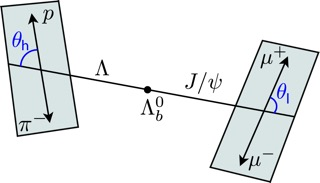
\includegraphics[width=0.5\textwidth]{Lmumu/figs/angles.jpeg}
\caption{Graphical representation of the angles for the \decay{\Lb}{\Lz\mumu} decay.}
\label{fig:Lb_angles}
\end{figure}

The $A_{\rm FB}^\ell$ observable is also measured in $\Bz\ra\Kstarz\mumu$ decays,
going through the same quark traditions as $\Lb\to\Lz\mumu$ decays. Instead the hadronic
asymmetry, $A_{\rm FB}^h$, is interesting only in the \Lb case as it is zero by definition
in \Bz decays where \Kstarz decays strongly.

\section{One-dimensional angular distributions}

In this section the derivation of the functional form of the angular distributions 
as a function of the $\cos\theta_\ell$ and $\cos\theta_h$ which are used to measure
the observables. The content of this section is based on the calculations in Ref.~\cite{Gutsche:2013pp}. 
For unpolarised \Lb production,
%
% the most general angular distribution can be written as 
%\begin{eqnarray}
%\label{bjoint3}
%W(\theta_\ell,\theta_h,\chi)  &\propto& 
%\sum_{\lambda_1,\lambda_{2},\lambda_j,\lambda'_j,J,J',m,m',\lambda_{\Lambda},
%\lambda'_{\Lambda},\lambda_{p}} 
%h^{m}_{\lambda_1\lambda_2}(J)h^{m'}_{\lambda_1\lambda_2}(J')
%e^{i(\lambda_{j}-\lambda'_{j})\chi}
%\nonumber\\ 
%&\times&
%\delta_{\lambda_{j}-\lambda_{\Lambda},\lambda'_{j}-\lambda'_{\Lambda}}
%\delta_{JJ'}
%d^J_{\lambda_j,\lambda_1-\lambda_{2}}(\theta_\ell)
%d^{J'}_{\lambda'_j,\lambda_1-\lambda_{2}}(\theta_\ell)
%H^{m}_{\lambda_{\Lambda}\lambda_{j}}(J)
%H^{m'\dagger}_{\lambda'_{\Lambda}\lambda'_{j}}(J')
%\nonumber \\
%&\times& 
%d^{1/2}_{\lambda_{\Lambda}\lambda_{p}}(\theta_h)
%d^{1/2}_{\lambda'_{\Lambda}\lambda_{p}}(\theta_h)
%h^{B}_{\lambda_{p}0}h^{B\,\dagger}_{\lambda_{p}0}\,.
%\end{eqnarray}
%where $\theta_\ell$, $\theta_h$ correspond to lepton and proton helicity angle, $\chi$ is angle between
%dimuon and \Lz decay planes (for unpolarized production we are sensitive only to difference in
%azimuthal angles), $d^J_{i,j}$ are Wigner d-functions and $h$, $h^B$ and $H$ are helicity amplitudes
%for virtual dimuon, \Lz and \Lb decays.
%The sum runs over all possible helicities with the dimuon being allowed in spin 0 and 1 states 
%($J$ and $J'$). The indeces $m$ and $m'$ run over the vector and axial-vector current contributions.
%
%Substituting for the dimuon amplitudes and integrating over three angles, one can obtain the differential
%branching fraction (eq. $11$ in Ref.~\cite{Gutsche:2013pp})
integrating over three angles the differential branching fraction is given in Eq. 11 of Ref.~\cite{Gutsche:2013pp} as
\begin{eqnarray}
\label{bjoint00}
\frac{d\Gamma(\Lambda_b \to \Lambda \,\ell^{+}\ell^{-})}{d q^2}=
\frac{v^{2}}{2}\cdot\bigg( U^{11+22} + L^{11+22} \bigg)
+\frac{2m_\ell^{2}}{q^{2}}\cdot\frac{3}{2}\cdot
\bigg( U^{11} + L^{11} + S^{22} \bigg)\,, 
\end{eqnarray}
%where we have adopted the notations
%$d\Gamma_X^{mm'}/d q^2=X^{mm'}$ and $X^{11+22}=X^{11}+X^{22}$.
%The bilinear expressions $H^{mm'}_{X}$ ($X=U,L,S$) are defined by
%\begin{equation}
%\label{helcom2}
%\qquad
%\begin{array}{lr}
%\mbox{$ H^{mm'}_U = 
%{\rm Re}(H^{m}_{\frac{1}{2}1} H^{\dagger m'}_{\frac{1}{2}1}) + 
%{\rm Re}(H^{m}_{-\frac{1}{2}-1} H^{\dagger m'}_{-\frac{1}{2}-1}) $}  & 
%\hfill\mbox{ \rm unpolarized-transverse}\,, 
%\\
%\mbox{$ H^{mm'}_L = 
%{\rm Re}(H^{m}_{\frac{1}{2}0} H^{\dagger m'}_{\frac{1}{2}0}) + 
%{\rm Re}(H^{m}_{-\frac{1}{2}0} H^{\dagger m'}_{-\frac{1}{2}0}) $}     & 
%\hfill\mbox{ \rm longitudinal}\,, 
%\\
%\mbox{$ H^{mm'}_S =  
%{\rm Re}(H^{m}_{\frac{1}{2}t}H^{\dagger m'}_{\frac{1}{2}t}) +  
%{\rm Re}(H^{m}_{-\frac{1}{2}t}H^{\dagger m'}_{-\frac{1}{2}t})$} &  
%\hfill\mbox{ \rm scalar}\,. 
%\end{array}\\
%\end{equation}
and the lepton helicity angle $\theta_\ell$ distribution is given in Eq. 15 as
\begin{eqnarray}
\label{costheta2}
\frac{d\Gamma(\Lambda_{b}\to \Lambda \,\ell^{+}\ell^{-})}{dq^2d\cos\theta_\ell} 
&=&\,
v^{2}\cdot\bigg[\frac{3}{8}\,(1+\cos^2\theta_\ell)\cdot
\frac{1}{2} U^{11+22}  
\ + \ \frac{3}{4}\,\sin^2\theta_\ell\cdot
\frac{1}{2} L^{11+22} \bigg]\label{distr2}\nonumber\\[2mm]
&-&\,v \cdot\frac{3}{4}\cos\theta_\ell\cdot P^{12} 
\ + \ \frac{2m_{\ell}^{2}}{q^{2}}\cdot \frac{3}{4}\cdot
\bigg[ U^{11}+ L^{11} + S^{22} \bigg]\,.
\end{eqnarray}
%Here in addition to amplitudes combinations entering differential branching fraction one more
%parity--odd term contributes
%\begin{equation}
%\label{helcom2a}
%\qquad\begin{array}{lr}
%\mbox{$H^{mm'}_P =  
%{\rm Re}(H^{m}_{\frac{1}{2}1}H^{\dagger m'}_{\frac{1}{2}1})- 
%{\rm Re}(H^{m}_{-\frac{1}{2}-1}H^{\dagger m'}_{-\frac{1}{2}-1})$} & 
%\hfill\mbox{ \rm parity--odd}
%\\
%\end{array}\\
%\end{equation}
%
In these formulas $m_\ell$ is the mass of the lepton and $v = \sqrt{1-4m_\ell^2/\qsq}$, $U$ denotes
the unpolarised-transverse contributions, $L$ the longitudinal
contributions and $S$ the scalar contribution. The apices $^{11}$ and $^{22}$ represent respectively
vector and axial-vector currents, with $X^{11+22} = X^{11} + X^{22}$.
The authors of Ref.~\cite{Gutsche:2013pp} define then the lepton-side forward-backward asymmetry as
\begin{equation}
A_{\rm FB}^{\ell}(q^{2}) 
= - \frac{3}{2}\,\frac{v\cdot P^{12}}
{v^{2}\cdot\big(\,U^{11+22}
+L^{11+22}\big)+\frac{2m_{\ell}^{2}}{q^{2}}\cdot 3 \cdot
\big(U^{11}+L^{11}
+S^{22}\,\big) }\,.
\label{eq:afbDef}
\end{equation}
%
%
%
Using these results as a starting point one can rewrite Eq.~\ref{costheta2} as
\begin{align}
\frac{d\Gamma(\Lambda_{b}\to \Lambda \,\ell^{+}\ell^{-})}{dq^2d\cos\theta_\ell}=&
\frac{3}{8}\frac{d\Gamma}{dq^2}\left(1+\cos^2\theta_\ell\right)U^{11+22}+
\frac{d\Gamma}{dq^2}A_{\rm FB}^\ell\cos\theta_\ell+
\frac{3}{8}\sin^2\theta_\ell v^2\left(L^{11+22}\right) \nonumber \\
&\left(U^{11}+L^{11}+S^{22}\right)\frac{3m_\ell^2}{q^2}\left(\frac{1}{8}-\frac{3}{8}\cos^2\theta_\ell\right)
\end{align}
 %
For this analysis the massless leptons limits is used, $m_\ell \rightarrow 0$. This is a good
approximation except at very low \qsq. In the massless limit the differential rates simplify to
\begin{eqnarray}
%\frac{d\Gamma(\Lambda_b \to \Lambda \,\ell^{+}\ell^{-})}{d q^2}=
\frac{d\Gamma}{d q^2}=
\frac{v^{2}}{2}\cdot\bigg( U^{11+22} + L^{11+22} \bigg)
\label{eq:totalBR}
\end{eqnarray}
and
\begin{align}
%\frac{d\Gamma(\Lambda_{b}\to \Lambda \,\ell^{+}\ell^{-})}{dq^2d\cos\theta_\ell}=&
\frac{d\Gamma}{dq^2d\cos\theta_\ell}=&
\frac{3}{8}\frac{d\Gamma}{dq^2}\left(1+\cos^2\theta_\ell\right)U^{11+22}+
\frac{d\Gamma}{dq^2}A_{FB}^\ell\cos\theta_\ell+
\frac{3}{8}\sin^2\theta_\ell v^2\left(L^{11+22}\right).
\label{eq:differentialBR}
\end{align}
%
%
Equations~\ref{eq:totalBR} and \ref{eq:differentialBR} can be then combined to achieve the form
\begin{align}
%\frac{d\Gamma(\Lambda_{b}\to \Lambda \,\ell^{+}\ell^{-})}{dq^2d\cos\theta_\ell}=
\frac{d\Gamma}{dq^2d\cos\theta_\ell}=
\frac{d\Gamma}{dq^2}&\left[
\frac{3}{8}\left(1+\cos^2\theta_\ell\right)\frac{U^{11+22}}{U^{11+22}+L^{11+22}}+A_{\rm FB}^\ell\cos\theta_\ell\right . +
 \nonumber \\
& \left. \frac{3}{4}\sin^2\theta_\ell\frac{L^{11+22}}{U^{11+22}+L^{11+22}}\right].
\end{align}
The amplitude combination in the last term can be viewed as ratio between longitudinal and sum of
longitudinal and unpolarized transverse contributions and therefore one can define the longitudinal fraction
\begin{equation}
f_{\rm L}=\frac{L^{11+22}}{U^{11+22}+L^{11+22}},
\end{equation}
which leads to the distribution used in the analysis
\begin{align}
%\frac{d\Gamma(\Lambda_{b}\to \Lambda \,\ell^{+}\ell^{-})}{dq^2d\cos\theta_\ell}=
\frac{d\Gamma}{dq^2d\cos\theta_\ell}=
\frac{d\Gamma}{dq^2}&\left[  \frac{3}{8}\left(1+\cos^2\theta_\ell\right)(1-f_L)+A_{\rm FB}^\ell\cos\theta_\ell +
   \frac{3}{4}\sin^2\theta_\ell f_{\rm L}\right]. 
   \label{eq:afbLTh}
\end{align}

Using the same steps the proton helicity distribution is given in Ref.~\cite{Gutsche:2013pp} as
\begin{equation}
\frac{d\Gamma(\Lambda_{b}\to \Lambda(\to p \pi^{-})\ell^{+}\ell^{-})}
     {dq^2\,d\cos\theta_h} 
={\rm Br}(\Lambda \to p\pi^{-})
 \frac{d\Gamma(\Lambda_b \to \Lambda\, \ell^{+}\ell^{-})}{d q^2}
\Big(\frac{1}{2}+A_{\rm FB}^h\cos\theta_h\Big) \,,
\label{eq:afbBTh}
\end{equation}
where 
\begin{equation}
A_{\rm FB}^h=\frac{1}{2}\alpha_{\Lz}P_z^\Lz(q^2).
\end{equation} 
where $P_z^\Lz(q^2)$ is the polarisation of the daughter baryon, \Lz,
and $\alpha_{\Lz} = 0.642 \pm 0.013$~\cite{PDG2014} is the \Lz decay asymmetry parameter.

%is defined as (eq.~$21$ in Ref.~\cite{Gutsche:2013pp})
%\begin{equation}
%\label{pz1}
%P_{z}^{\Lambda}=\frac{
%v^{2}\cdot\big(\,P^{11+22}
%+L_{P}^{11+22}\big)+\frac{2m_{\ell}^{2}}{q^{2}}\cdot 3 \cdot 
%\big(P^{11}+L_{P}^{11}
%+S_{P}^{22}\,\big)
%}
%{v^{2}\cdot\big(\,U^{11+22}
%+L^{11+22}\big)+\frac{2m_{\ell}^{2}}{q^{2}}\cdot 3 \cdot
%\big(U^{11}+L^{11}
%+S^{22}\,\big) 
%} \,.
%\end{equation}

%where two parity-violating combinations of amplitudes
%\begin{equation}
%\label{helcom3}
%\qquad\begin{array}{lr}
%\mbox{$H^{mm'}_{L_{P}}=
%{\rm Re}
%(H^{m}_{\frac{1}{2}\,0}H^{\dagger m'}_{\frac{1}{2}\,0}-H^{m}_{-\frac{1}{2}\,0}
%H^{\dagger m'}_{-\frac{1}{2}\,0})$} & 
%\hfill\mbox{ \rm longitudinal--polarized}\,, 
%\\
%\mbox{$H^{mm'}_{S_{P}}=
%{\rm Re}
%(H^{m}_{\frac{1}{2}\,t}H^{\dagger m'}_{\frac{1}{2}\,t}-H^{m}_{-\frac{1}{2}\,t}
%H^{\dagger m'}_{-\frac{1}{2}\,t})$}
% & 
%\hfill\mbox{ \rm scalar--polarized}\,, 
%\end{array}\\
%\end{equation}
%enter in addition to the ones we already discussed.

%While lepton side observables are well known from meson decays, hadron side is unexplored. To get
%feeling how sensitive $A_{FB}^h$ is to new physics, we plot together three different cases: first,
%SM using predictions and numerical values from Ref.~\cite{Gutsche:2013pp}, scenario in which Wilson
%coefficients are same as in the SM, just sign of the $C_7$ is flipped and finally modifying $C_7$,
%$C_9$ and $C_{10}$ by amount compatible with fit to meson data including $P_5'$ in
%Ref.~\cite{Descotes-Genon:2013wba}.
%Resulting dependence of $P_z^\Lz$ is shown in Fig.~\ref{fig:PzLpred}.
%
%\begin{figure}
%\centering
%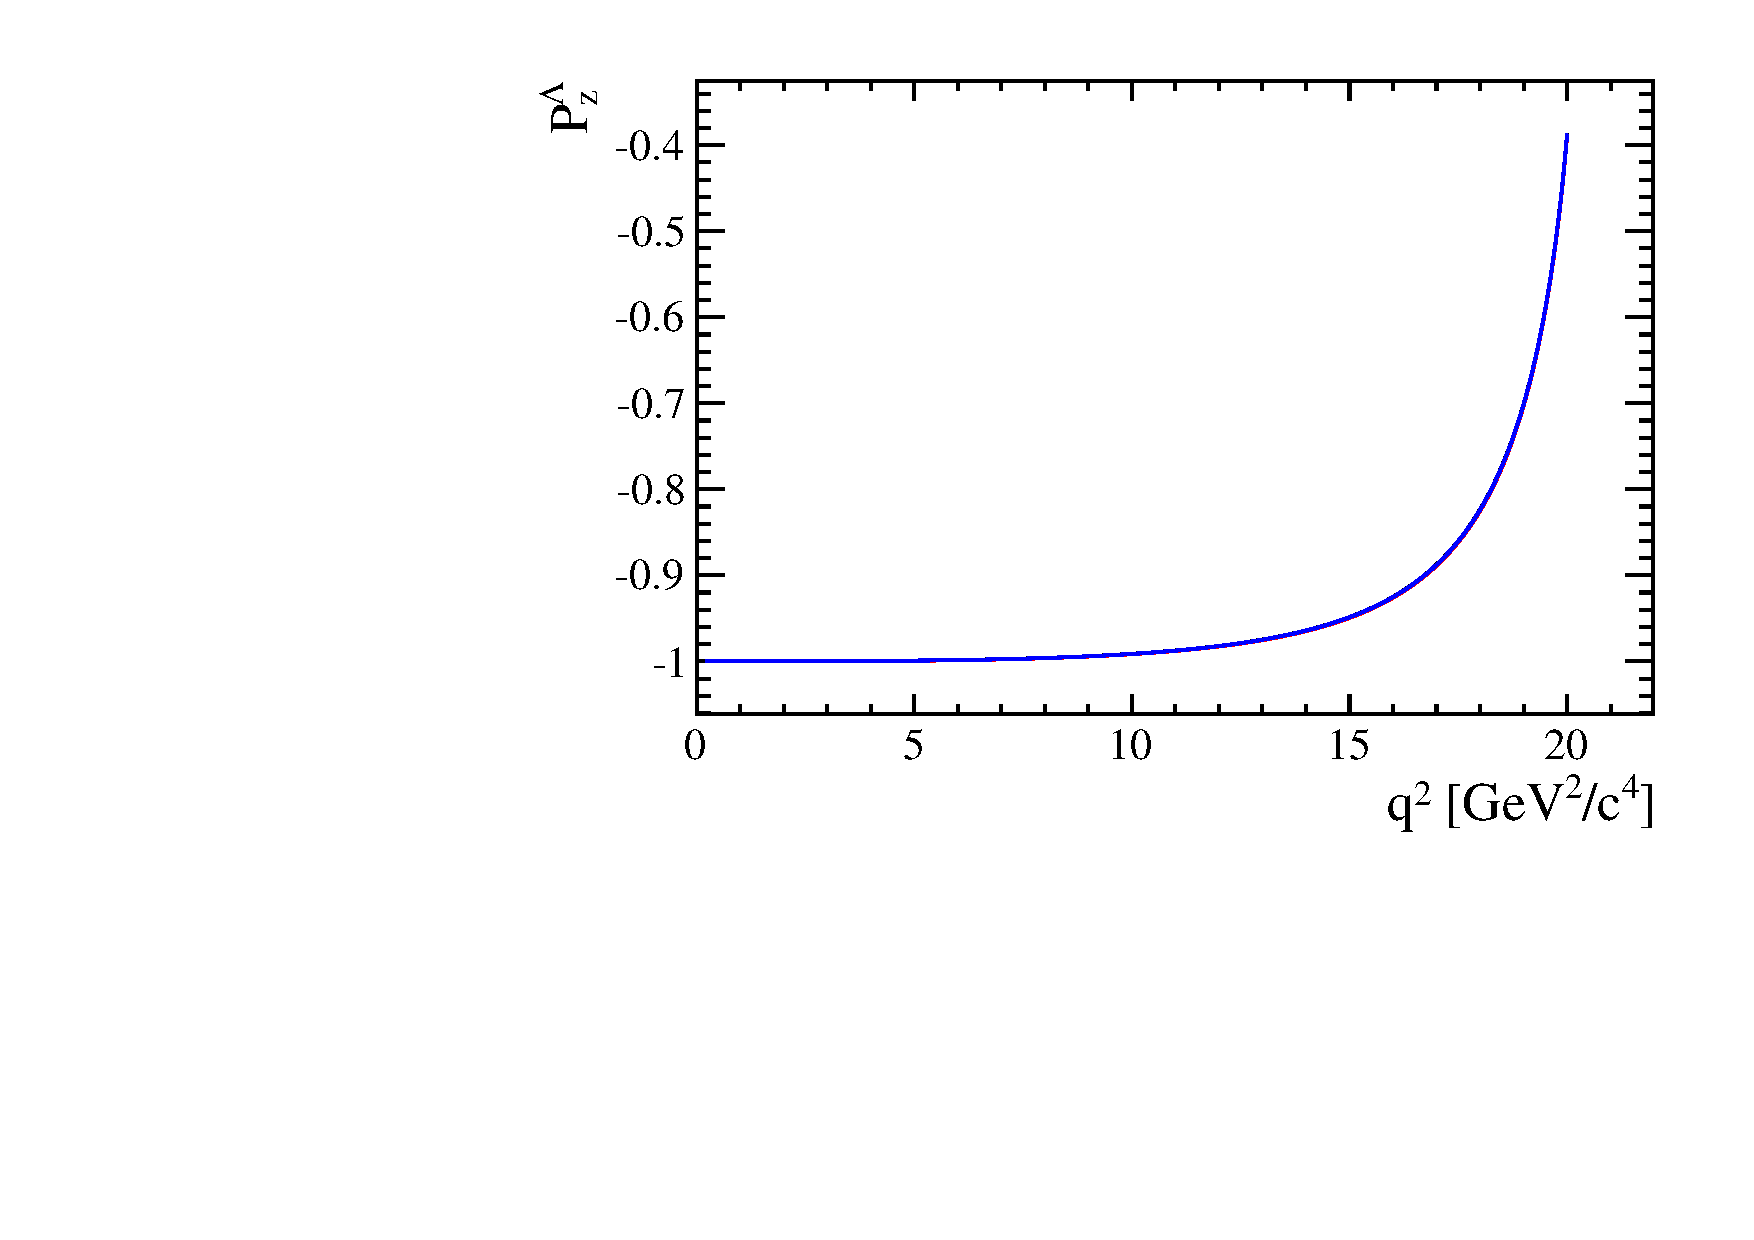
\includegraphics[width=0.7\textwidth]{Lmumu/figs/AFBhPrediction}
%\caption{Expectation for $P_z^\Lz$ which is proportional to $A_{FB}^h$ in the SM (black line), SM
%like scenario with flipped sign on $C_7$ (red line) and scenario with all three Wilson coefficients
%modified according to Ref.~\cite{Descotes-Genon:2013wba} (blue line). There is little difference
%between those tree scenarious.}
%\label{fig:PzLpred}
%\end{figure}
%
%As can be seen, there is little difference between three scenarious. We also tried to investigate
%analytically. In that case we put lepton mass to zero and neglect $C_7$ terms, which are small at
%high $q^2$ where we have most of the signal. In such case, both numerator and denumerator in
%eq.~\ref{pz1} are proportional to $(|C_9|^2+|C_{10}|^2)$ and thus dependence on Wilson coefficients
%drops out in first order. So only difference can come from $C_7$ and its interference with other two Wilson
%coefficients and thus effects are expected to be small. From this we conclude that main help of this
%variable is in constraining form factors in the studied decay. 


These expressions assume that \Lb is produced unpolarised, which is in agreement with the recent LHCb
measurement of the production polarisation~\cite{LHCb-PAPER-2012-057}.
Possible effects due to a non zero production polarisation are investigated in systematic uncertainties.


\section{Multi-dimensional angular distributions}

To incorporate effects of production polarisation this was introduced in the equations.
%
%, we modify Eq.~\ref{bjoint3} to  
%\begin{eqnarray}
%\label{bjoint4}
%W(\theta,\theta_\ell,\phi_\ell,\theta_h,\phi_\Lambda)  &\propto& 
%\sum_{\lambda_1,\lambda_{2},\lambda_j,\lambda'_j,J,J',m,m',\lambda_{\Lambda},
%\lambda'_{\Lambda},\lambda_{p}} 
%h^{m}_{\lambda_1\lambda_2}(J)h^{m'}_{\lambda_1\lambda_2}(J')
%\rho_{\lambda_{j}-\lambda_{\Lambda},\lambda'_{j}-\lambda'_{\Lambda}}(\theta)
%(-1)^{J+J'}
%\nonumber\\ 
%&\times&D^J_{\lambda_j,\lambda_1-\lambda_{2}}(\theta_\ell,\phi_\ell)
%D^{J'}_{\lambda'_j,\lambda_1-\lambda_{2}}(\theta_\ell,\phi_\ell)
%H^{m}_{\lambda_{\Lambda}\lambda_{j}}(J)
%H^{m'\dagger}_{\lambda'_{\Lambda}\lambda'_{j}}(J')
%\nonumber \\
%&\times& 
%D^{1/2}_{\lambda_{\Lambda}\lambda_{p}}(\theta_h,\phi_\Lambda)
%D^{1/2}_{\lambda'_{\Lambda}\lambda_{p}}(\theta_h,\phi_\Lambda)
%h^{B}_{\lambda_{p}0}h^{B\,\dagger}_{\lambda_{p}0}\,,
%\end{eqnarray}
%where
%\begin{equation}
%D^{J}_{m,n}(\theta_i,\phi_i)=e^{-i(m-n)\phi_i}d^J_{m,n}(\theta_i).
%\end{equation}
In the modified version, the angle $\theta$ is sensitive to the production polarisation
through the spin-density matrix in Eq.~\ref{eq:spinDensity}. 
%, while the angle between the decay planes $\chi$ is changed to the polar angles of proton and positive muon.
Integrating over $\theta_h$, $\phi_\Lambda$, $\phi_\ell$ and $\theta$ results in 
the same distribution as in the unpolarised case (Eq.~\ref{costheta2}). Therefore, in the case of uniform
efficiency, the lepton side forward-backward asymmetry, $A_{FB}^\ell$, is unaffected by production
polarisation. To estimate effect of the production polarisation, the two-dimensional
distribution in $\theta$ and $\theta_\ell$ is also derived, which in the massless leptons
limit becomes (up to a  constant multiplicative factor)
%
\begin{align}
\frac{d\Gamma(\Lambda_{b}\to \Lambda \,\ell^{+}\ell^{-})}{dq^2d(\cos\theta) d(\cos\theta_\ell)}=&
\frac{d\Gamma}{dq^2}\left\{  \frac{3}{8}\left(1+\cos^2\theta_\ell\right)(1-f_L)+A_{FB}^\ell\cos\theta_\ell +
   \frac{3}{4}\sin^2\theta_\ell f_L+\right. \nonumber \\
&P_b\cos(\theta)\left[ -\frac{3}{4}\sin(\theta_\ell)^2O_{Lp}+
  \frac{3}{8}\left(1+\cos(\theta_\ell)^2\right)O_P\right. \nonumber \\
&\left.\left.-\frac{3}{8}\cos(\theta_\ell)O_{U12} \right]\right\}\,,
\label{eq:lepton2D}
\end{align}
where three more observables are defined
\begin{align}
O_{Lp}=&\frac{L_P^{11}+L_P^{22}}{U^{11+22}+L^{11+22}}, \nonumber \\
O_P=&\frac{P^{11}+P^{22}}{U^{11+22}+L^{11+22}}, \nonumber \\
O_{U12}=&\frac{U^{12}}{U^{11+22}+L^{11+22}}. \nonumber
\end{align}
%
In the massless leptons approximation two of these quantities are related to hadron side
forward-backward asymmetry as
\begin{equation}
\frac{1}{2}\alpha_\Lambda \left(O_P+O_{Lp}\right)=A_{FB}^h\,.
\end{equation}
%
Following the same steps as lepton side case, after integrating over four angles one finds that
the hadron side, $A_{FB}^h$, is also unaffected by the production polarization in case of uniform
efficiency. The two dimensional distribution in $\theta$ and $\theta_h$ has form
\begin{align}
\frac{d\Gamma(\Lambda_{b}\to \Lambda \,\ell^{+}\ell^{-})}{dq^2d(\cos\theta) d(\cos\theta_B)}=
\frac{d\Gamma}{dq^2}&\left[1+2A_{FB}^h\cos\theta_B+P_b\left(O_P-O_{Lp}\right)\cos\theta\right.\nonumber \\
&\left.+\alpha_\Lz P_b\left(1-2f_L\right)\cos\theta\cos\theta_B\right].
\label{eq:hadron2D}
\end{align}

%It should be noted that fact that in case of uniform efficiency both angular observables are
%unaffected by production polarization comes from the fact that terms proportional to $\sin\theta$
%cancel out when integrating over $\phi_\ell$ and $\phi_\Lambda$ and remaining terms containing production
%polarization go as $\cos\theta$, which after integrating over it yields zero.
%
In order to use two-dimensional distributions, expectations for the three additional observables,
which do not enter one-dimensional distributions are needed.
Expectations are calculated using form factors and numerical inputs from Ref.~\cite{Gutsche:2013pp}
and are shown in Tab.~\ref{tab:obsGutsche1}.
%
%In this calculation the massless lepton limit
%is used and compared to the
%Ref.~\cite{Gutsche:2013pp} we turn off long-distance contributions by setting dileptonic decay
%widths of \jpsi and $\psi(2S)$ to zero. In order to obtain binned values, we need to integrate
%corresponding amplitudes over \qsq interval and this is done separately for those in the numerator
%and denominator rather than integrating ratio of amplitudes. Results are in tables
%\ref{tab:obsGutsche1}. Alternatively we calculate also expectation using lattice QCD form factors
%from Ref.~\cite{Detmold:2012vy} by substituting those instead of form factors from Ref.~\cite{Gutsche:2013pp}.
%These results are in table \ref{tab:lQCD1}.
%
\begin{table}
\begin{center}
\begin{tabular}{lcccccc}\hline
\qsq [$GeV^2/c^2$]  & $A_{FB}^\ell$ & $P_z^\Lz$  & $f_L$   & $O_P$  & $O_{Lp}$ & $O_{U12}$ \\ \hline
0.1 -- 2.0          &  0.082     & -0.9998    & 0.537   & -0.463 & -0.537   &  0.055  \\ 
2.0 -- 4.0          & -0.032     & -0.9996    & 0.858   & -0.142 & -0.857   & -0.021  \\ 
4.0 -- 6.0          & -0.153     & -0.9991    & 0.752   & -0.247 & -0.752   & -0.102  \\ 
11.0 -- 12.5        & -0.348     & -0.9834    & 0.508   & -0.478 & -0.505   & -0.239  \\ 
15.0 -- 16.0        & -0.384     & -0.9374    & 0.428   & -0.524 & -0.413   & -0.280  \\ 
16.0 -- 18.0        & -0.377     & -0.8807    & 0.399   & -0.513 & -0.368   & -0.294  \\ 
18.0 -- 20.0        & -0.297     & -0.6640    & 0.361   & -0.404 & -0.260   & -0.314  \\ \hline 
1.0 -- 6.0          & -0.040     & -0.9994    & 0.830   & -0.170 & -0.830   & -0.027  \\ 
15.0 -- 20.0        & -0.339     & -0.7830    & 0.385   & -0.461 & -0.322   & -0.302  \\ \hline
\end{tabular}
\end{center}
\caption{Prediction for angular observables entering two-dimensional angular distributions.
Prediction is based on covariant quark model form factors from Ref.~\cite{Gutsche:2013pp}.}
\label{tab:obsGutsche1}
\end{table}
%
%
%\begin{table}
%\begin{center}
%\begin{tabular}{lcccccc}\hline
%\qsq [$GeV^2/c^2$]  & $A_{FB}^\ell$ & $P_z^\Lz$  & $f_L$   & $O_P$  & $O_{Lp}$ & $O_{U12}$ \\ \hline
%0.1 -- 2.0          &  0.023     & -0.963    & 0.904   & -0.096 & -0.867   &  0.015  \\ 
%2.0 -- 4.0          & -0.085     & -0.962    & 0.870   & -0.128 & -0.834   & -0.058  \\ 
%4.0 -- 6.0          & -0.163     & -0.962    & 0.771   & -0.224 & -0.739   & -0.111  \\ 
%11.0 -- 12.5        & -0.316     & -0.934    & 0.541   & -0.427 & -0.507   & -0.227  \\ 
%15.0 -- 16.0        & -0.346     & -0.866    & 0.450   & -0.468 & -0.398   & -0.271  \\ 
%16.0 -- 18.0        & -0.336     & -0.799    & 0.416   & -0.455 & -0.344   & -0.288  \\ 
%18.0 -- 20.0        & -0.260     & -0.585    & 0.368   & -0.354 & -0.231   & -0.311  \\ \hline 
%1.0 -- 6.0          & -0.086     & -0.962    & 0.865   & -0.132 & -0.829   & -0.059  \\ 
%15.0 -- 20.0        & -0.306     & -0.721    & 0.402   & -0.415 & -0.306   & -0.295  \\ \hline
%\end{tabular}
%\end{center}
%\caption{Prediction for angular observables entering two-dimensional angular distributions.
%Prediction is based on lattice QCD form factors from Ref.~\cite{Detmold:2012vy}.}
%\label{tab:lQCD1}
%\end{table}

For completeness, the two-dimensional distribution in $\cos\theta_L$-$\cos\theta_B$ has the form
\begin{align}
\frac{d\Gamma(\Lambda_{b}\to \Lambda \,\ell^{+}\ell^{-})}{dq^2d(\cos\theta_B) d(\cos\theta_L)}=&
\frac{3}{8}+\frac{6}{16}\cos^2\theta_L(1-f_L)-\frac{3}{16}\cos^2\theta_L f_L
+A_{FB}^l\cos\theta_L+ \nonumber \\
& \left(\frac{3}{2}A_{FB}^h-\frac{3}{8}\alpha_\Lz O_P\right)\cos\theta_B
-\frac{3}{2}A_{FB}^h\cos^2\theta_L\cos\theta_B-\frac{3}{16}f_L+ \nonumber \\
& \frac{9}{16}f_L\sin^2\theta_L+\frac{9}{8}\alpha_\Lz \cos^2\theta_L\cos\theta_B O_P- \nonumber \\
& \frac{3}{2}\alpha_\Lz \cos\theta_L\cos\theta_B O_{U12}.
\label{eq:2DcosThetaLandB}
\end{align}
%It does not need any additional inputs compared to previous two-dimensional distributions.


\section{Angular resolution}
\label{sec:and_resolution}

In this section is reported a study of the angular resolution done in order to achieve a better understanding
of detector and reconstruction effects. This will be then used to study systematic uncertainties.
The study is done by analysing simulated events and comparing true and reconstructed quantities.
In Fig.~\ref{fig:resolutionvsq2ang} plots of the difference between true and measured angular observables 
($\cos \theta_\ell$ and $\cos \theta_h$)  are reported as a function of the observable itself.
These are centred at 0 indicating no bias in the measurement.
%Plots shown are done on long-long events only but we performed the same study separately on down-down events too.
In Fig.~\ref{fig:resolutionvsq2ang} the same difference is shown also as a function of \qsq showing again no bias.
The spread the distributions on these plots around the central value is an estimate of the angular resolution.
Taking vertical slices of the distributions in Fig.~\ref{fig:resolutionvsq2ang} approximately gaussian
distributions centred at 0 are obtained. These distributions are fit with a single gaussian and its $\sigma$
is interpreted as angular resolution. In Tab.~\ref{tab:resolutions} he average resolutions are reported
for the two angular variables separately for the long and downstream candidates. As expected candidates built
from long tracks are characterised by a better resolution due to a better momentum and vertex resolution.
%Furthermore also the resolution of the lepton observable is better than the hadronic one.
In Fig.~\ref{fig:avgResol} responce matrices, showing the correlation between reconstructed and
generated angular observables, are shown.

\begin{table}[b]
\centering
\caption{Average angular resolutions integrated over the full interval and the full available \qsq.}
\begin{tabular}{l|cc}
Observable      & DD & LL     \\ \hline
$\cos \theta_\ell$ & 0.015 & 0.01 \\
$\cos \theta_h$ & 0.066 & 0.014 \\
\end{tabular}
\label{tab:resolutions}
\end{table}


\begin{figure}
\centering
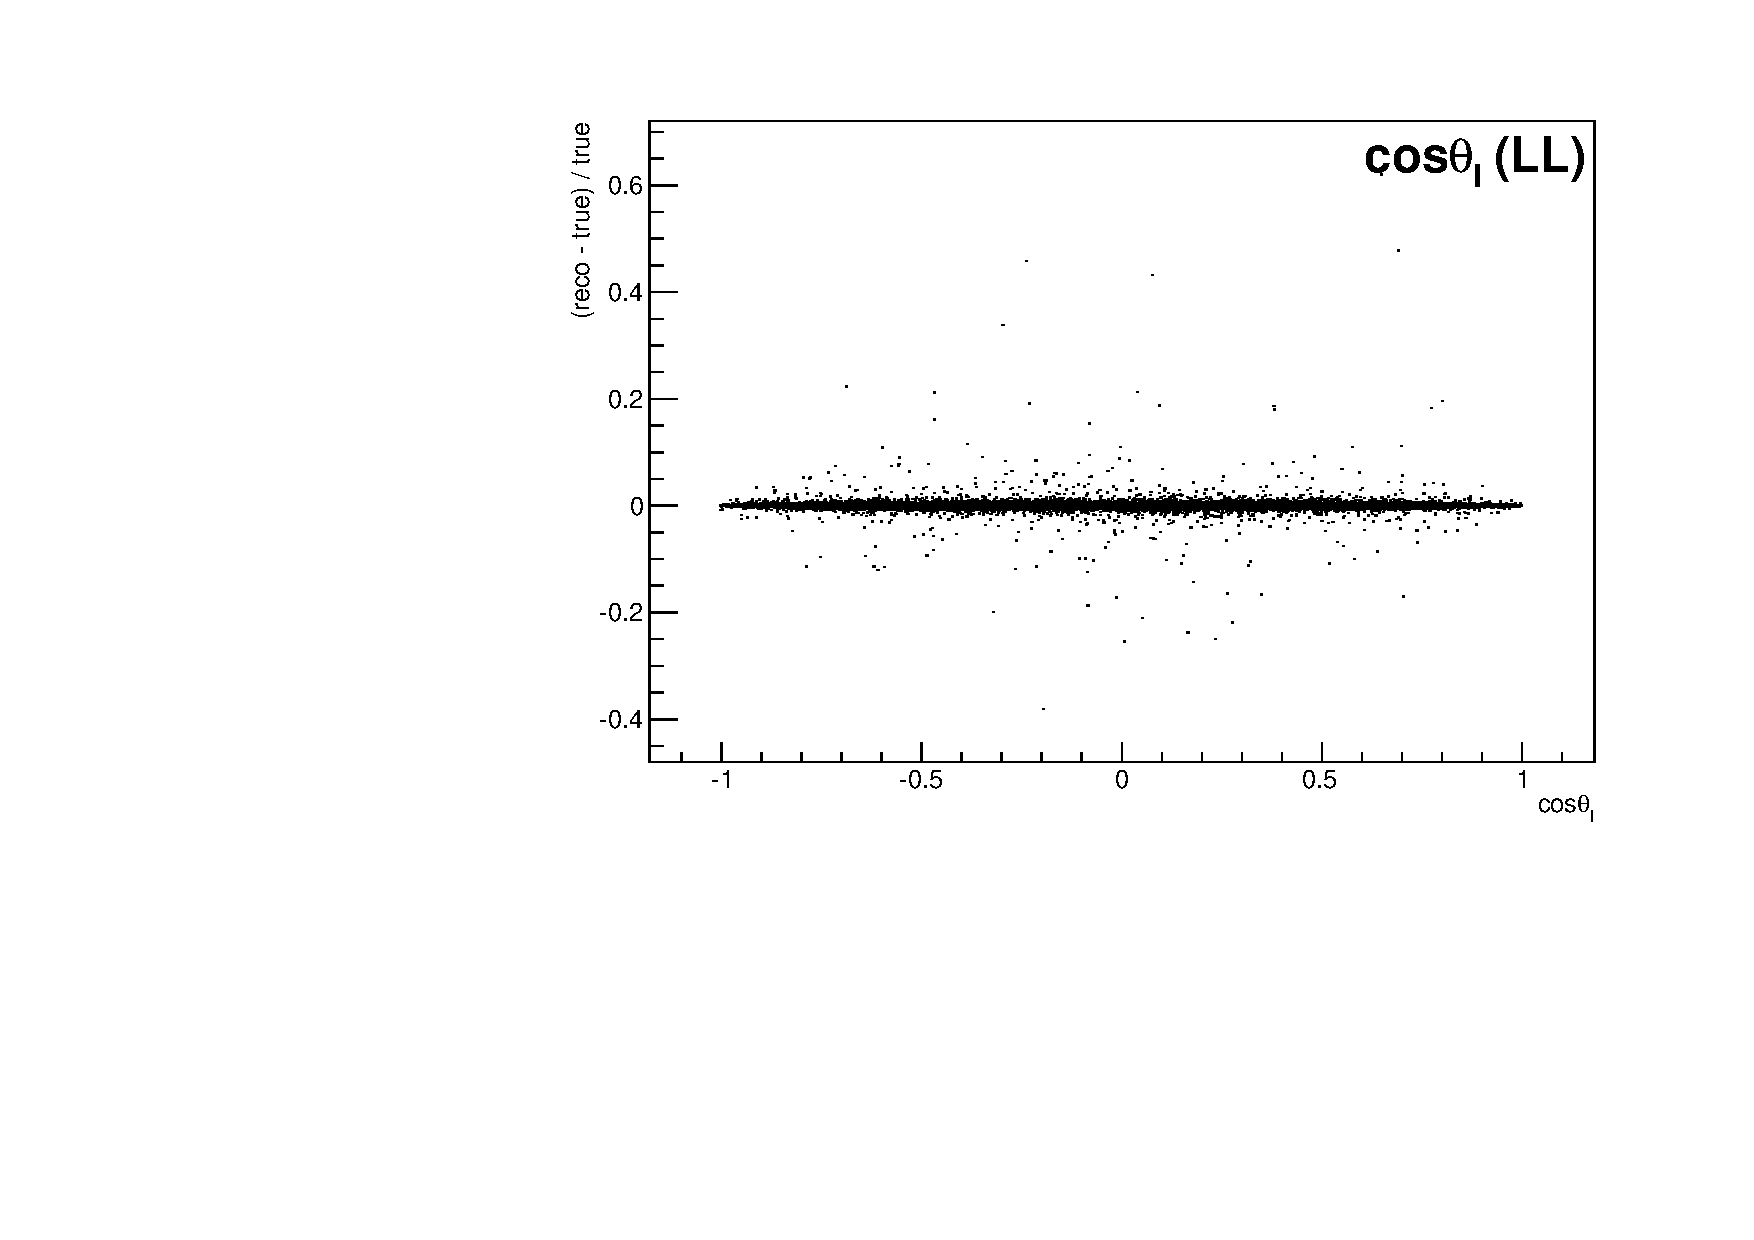
\includegraphics[width=0.48\textwidth]{Lmumu/figs/resolution/RmT_vs_cosThetaL_LL.pdf}
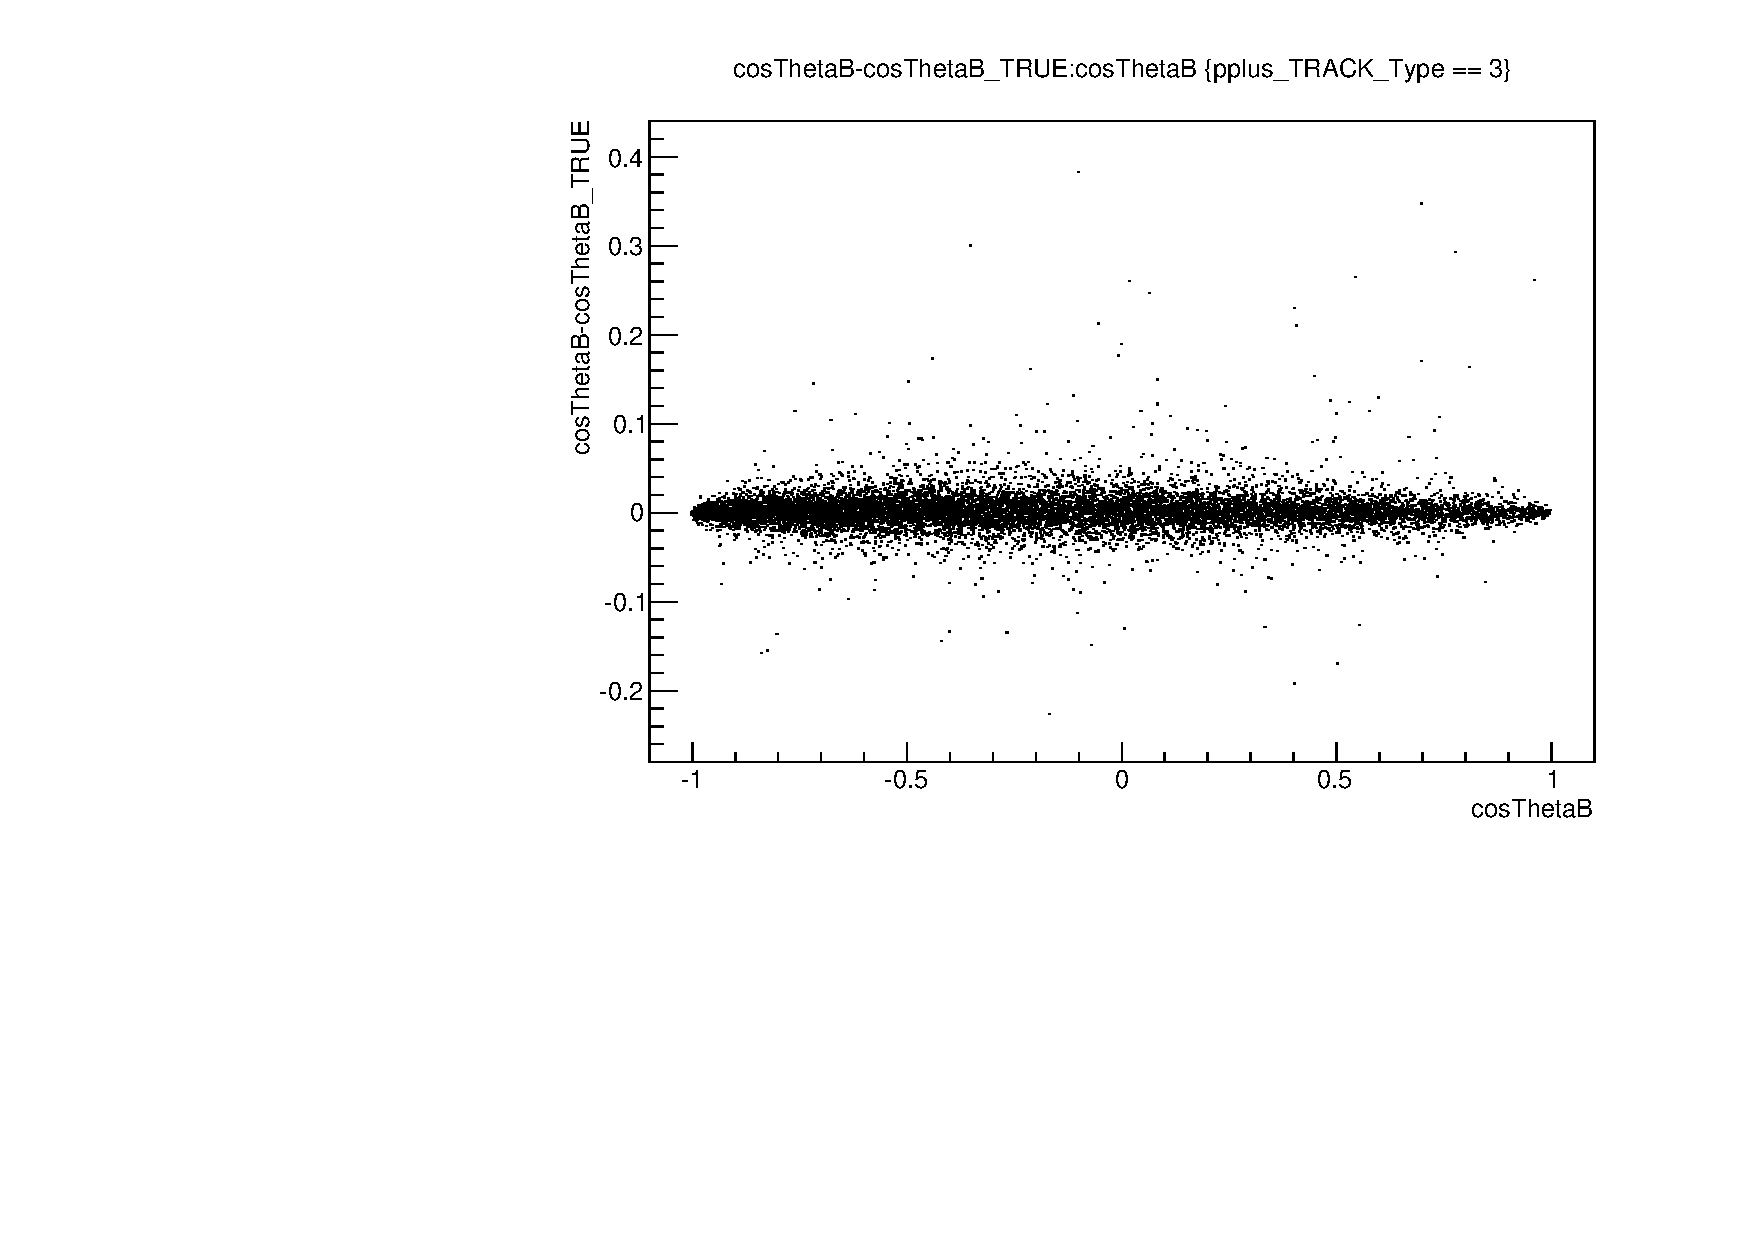
\includegraphics[width=0.48\textwidth]{Lmumu/figs/resolution/RmT_vs_cosThetaB_LL.pdf}
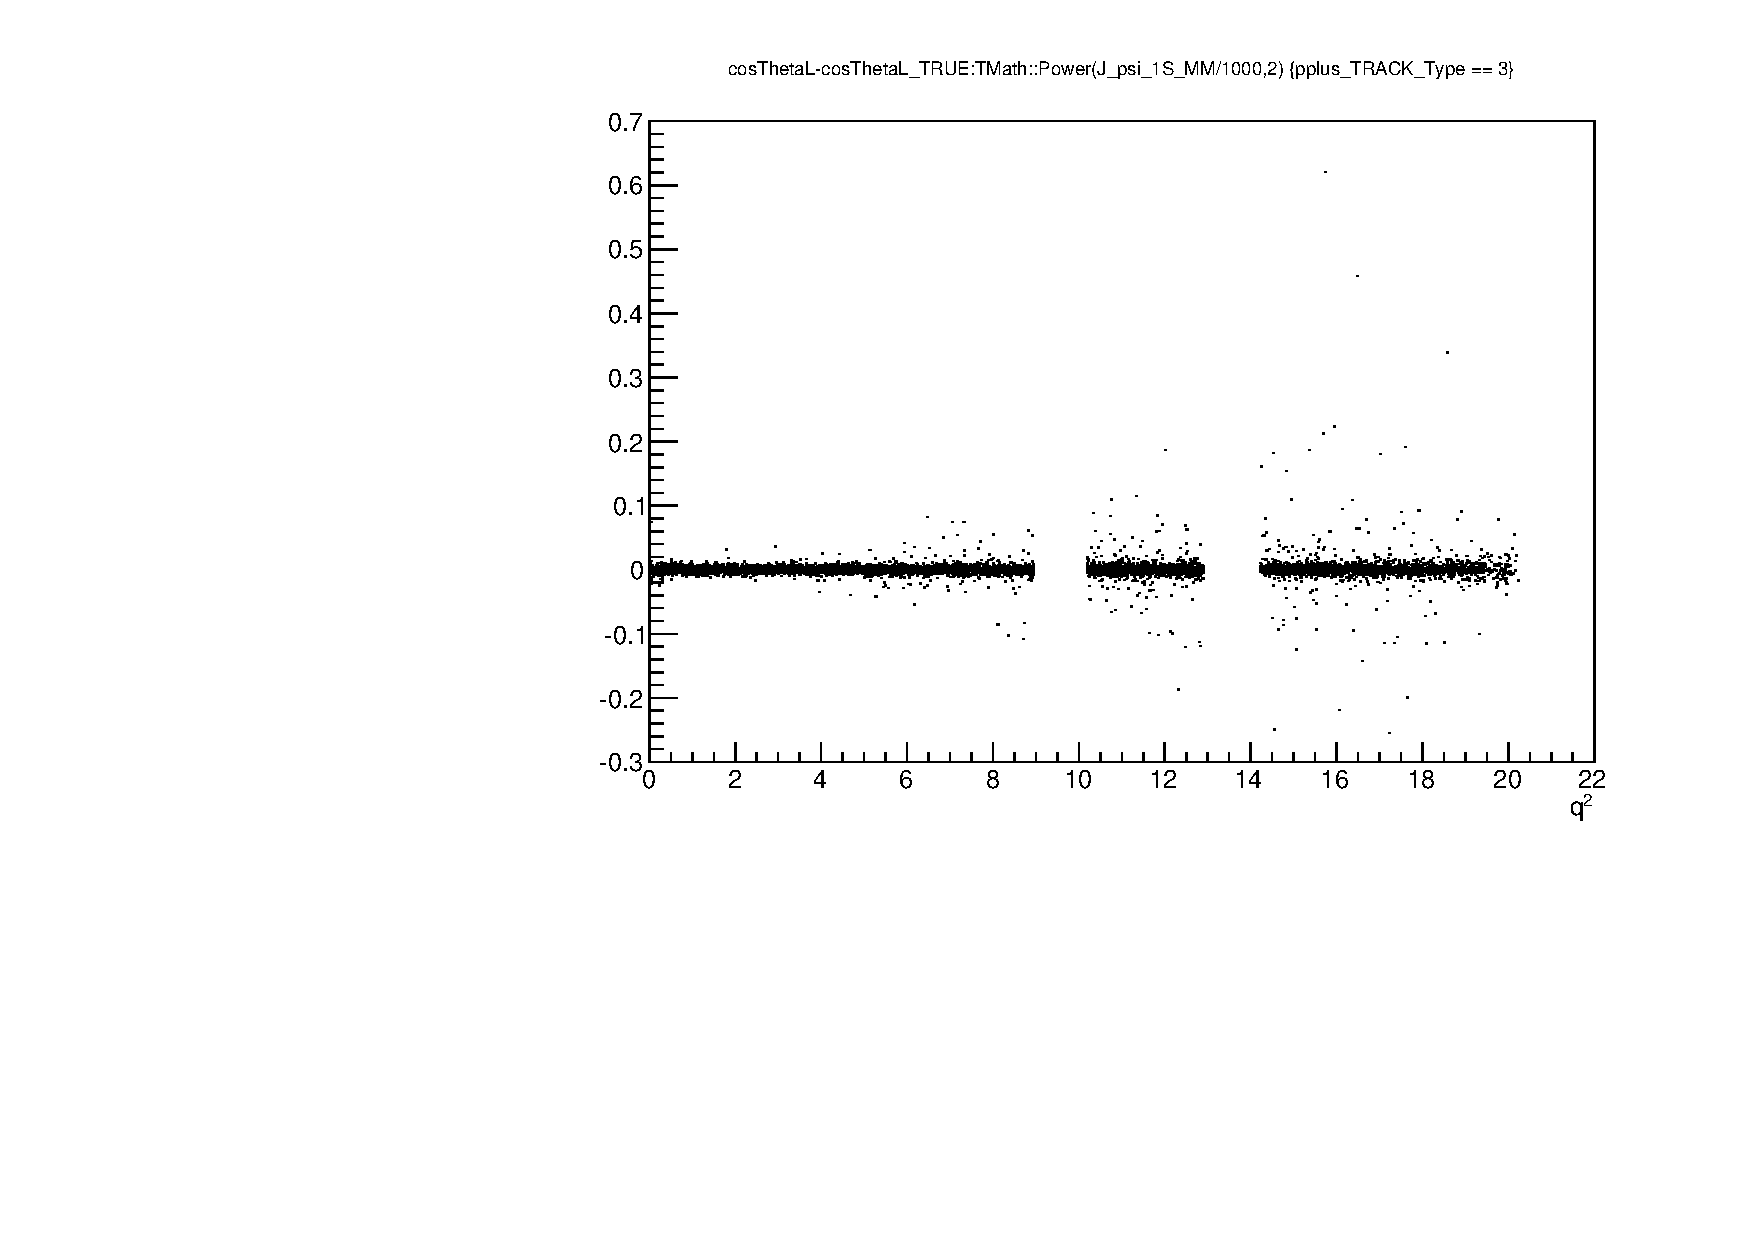
\includegraphics[width=0.48\textwidth]{Lmumu/figs/resolution/RmTcosThetaL_vs_q2_LL.pdf}
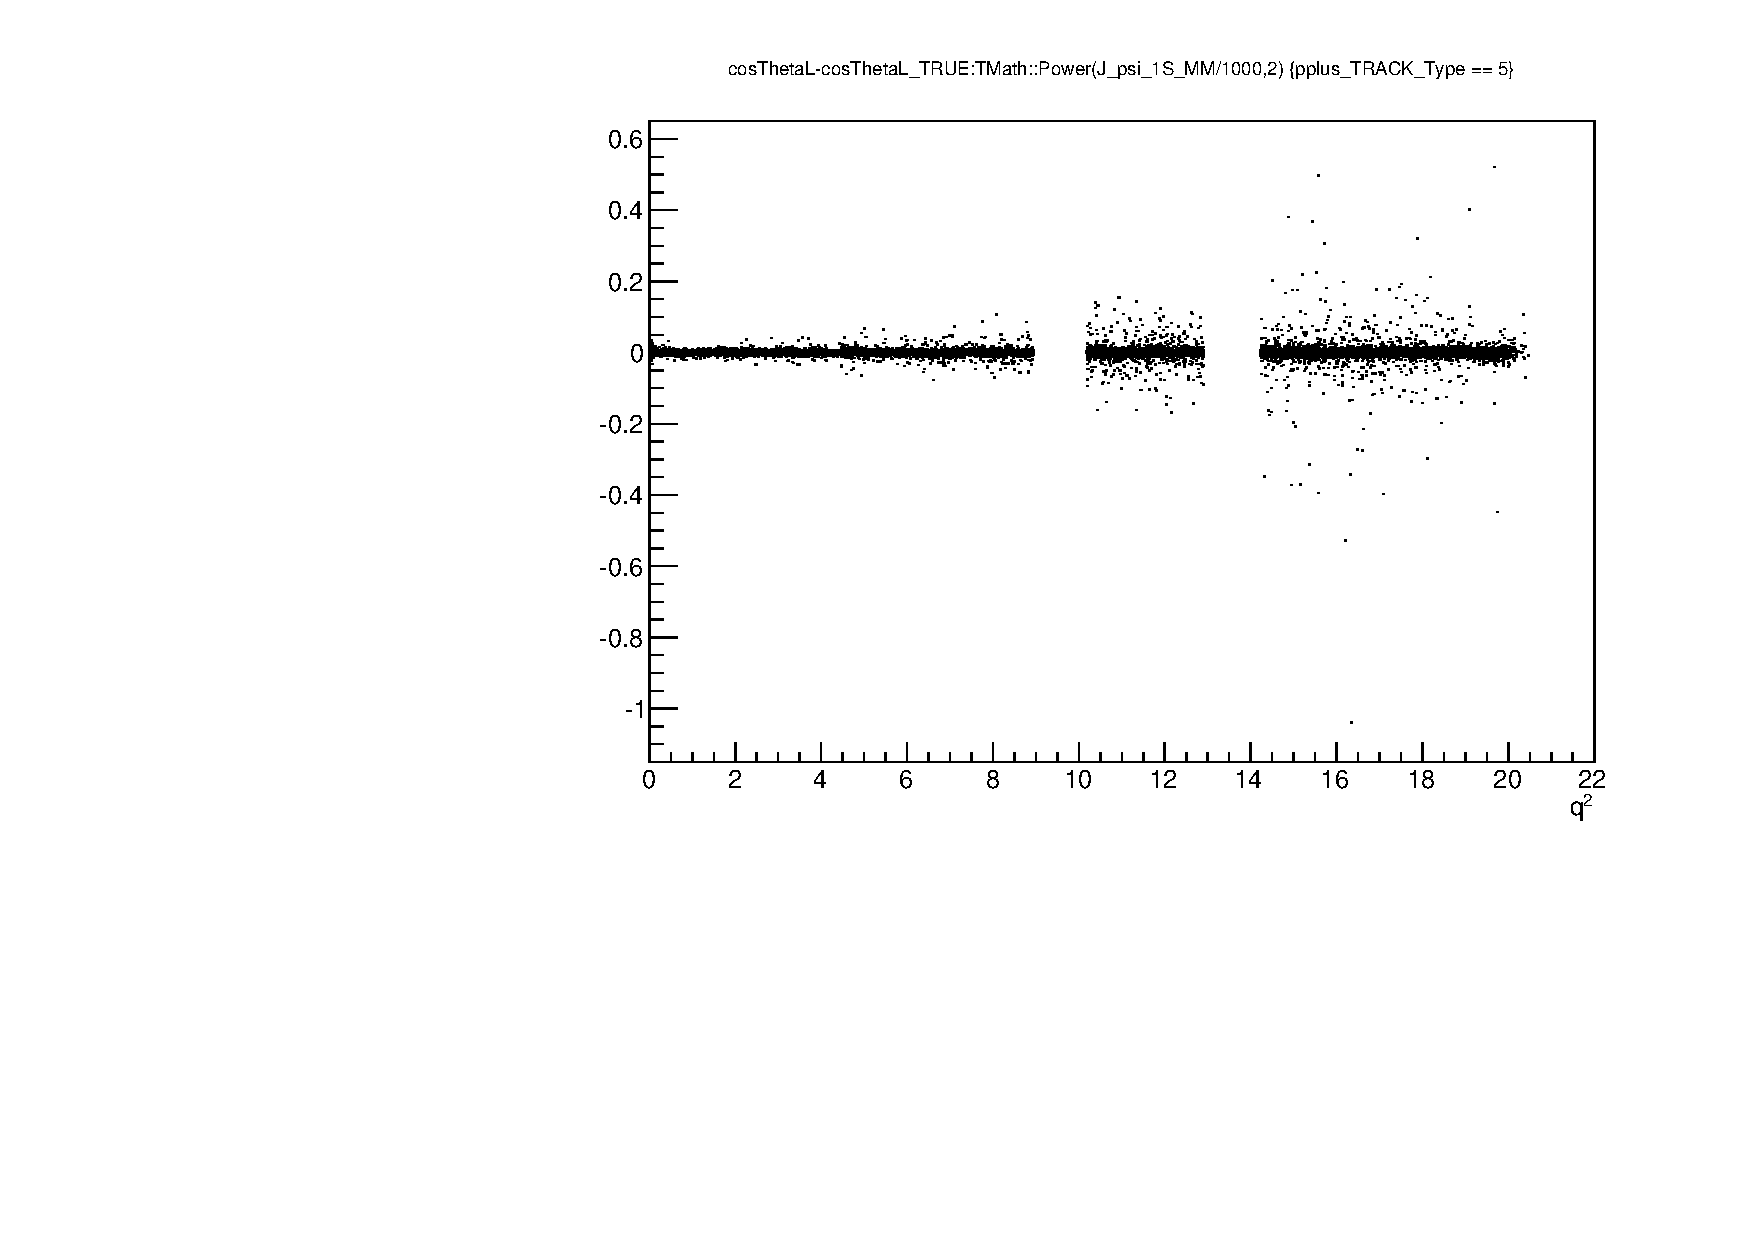
\includegraphics[width=0.48\textwidth]{Lmumu/figs/resolution/RmTcosThetaL_vs_q2_DD.pdf}
 \caption{Difference of between generated and reconstructed angular observables as a function of 
 the observables themselves (top) for long candidates and as a function of \qsq for 
 long (bottom left) and downstream (bottom right) candidates.}
\label{fig:resolutionvsq2ang}
\end{figure}

\begin{figure}
\centering
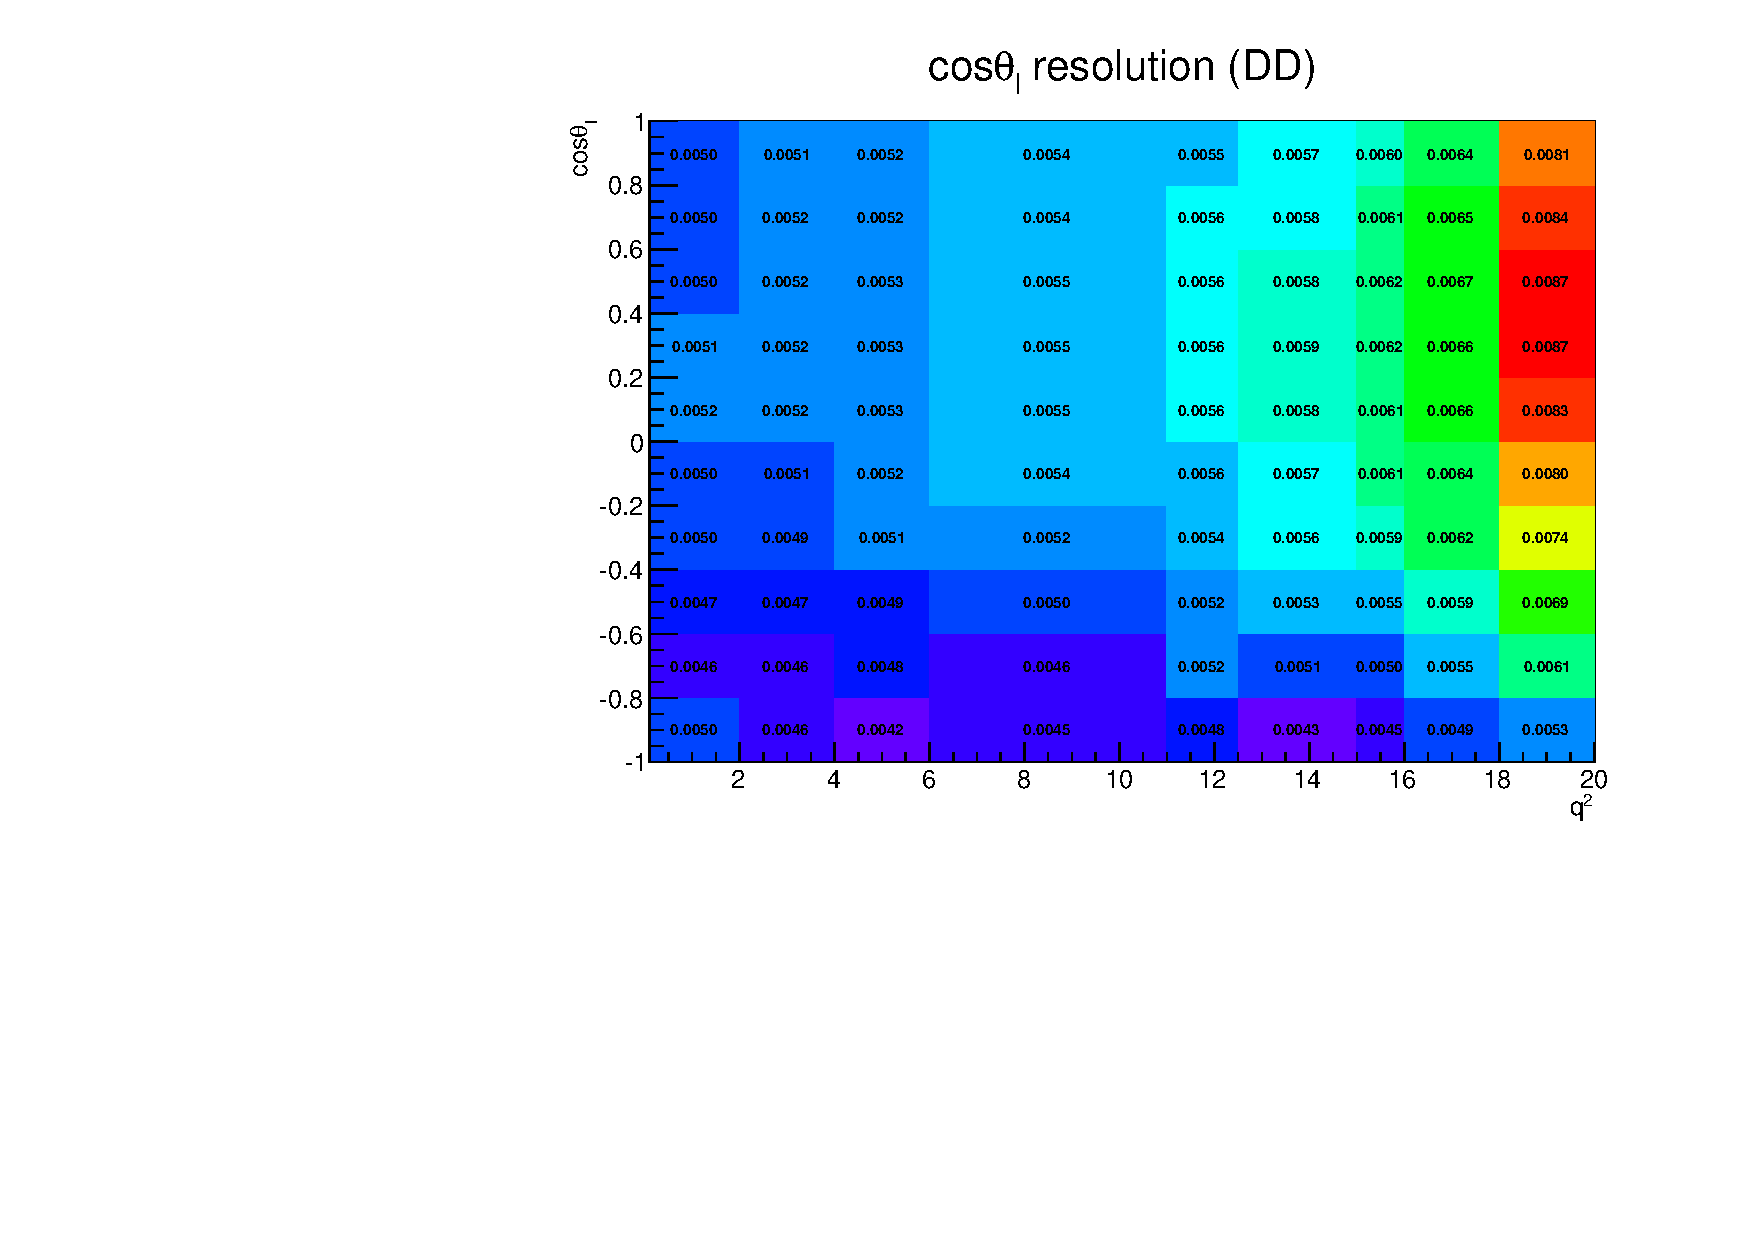
\includegraphics[width=0.48\textwidth]{Lmumu/figs/resolution/resolution2D_cosThetaL_DD.pdf}
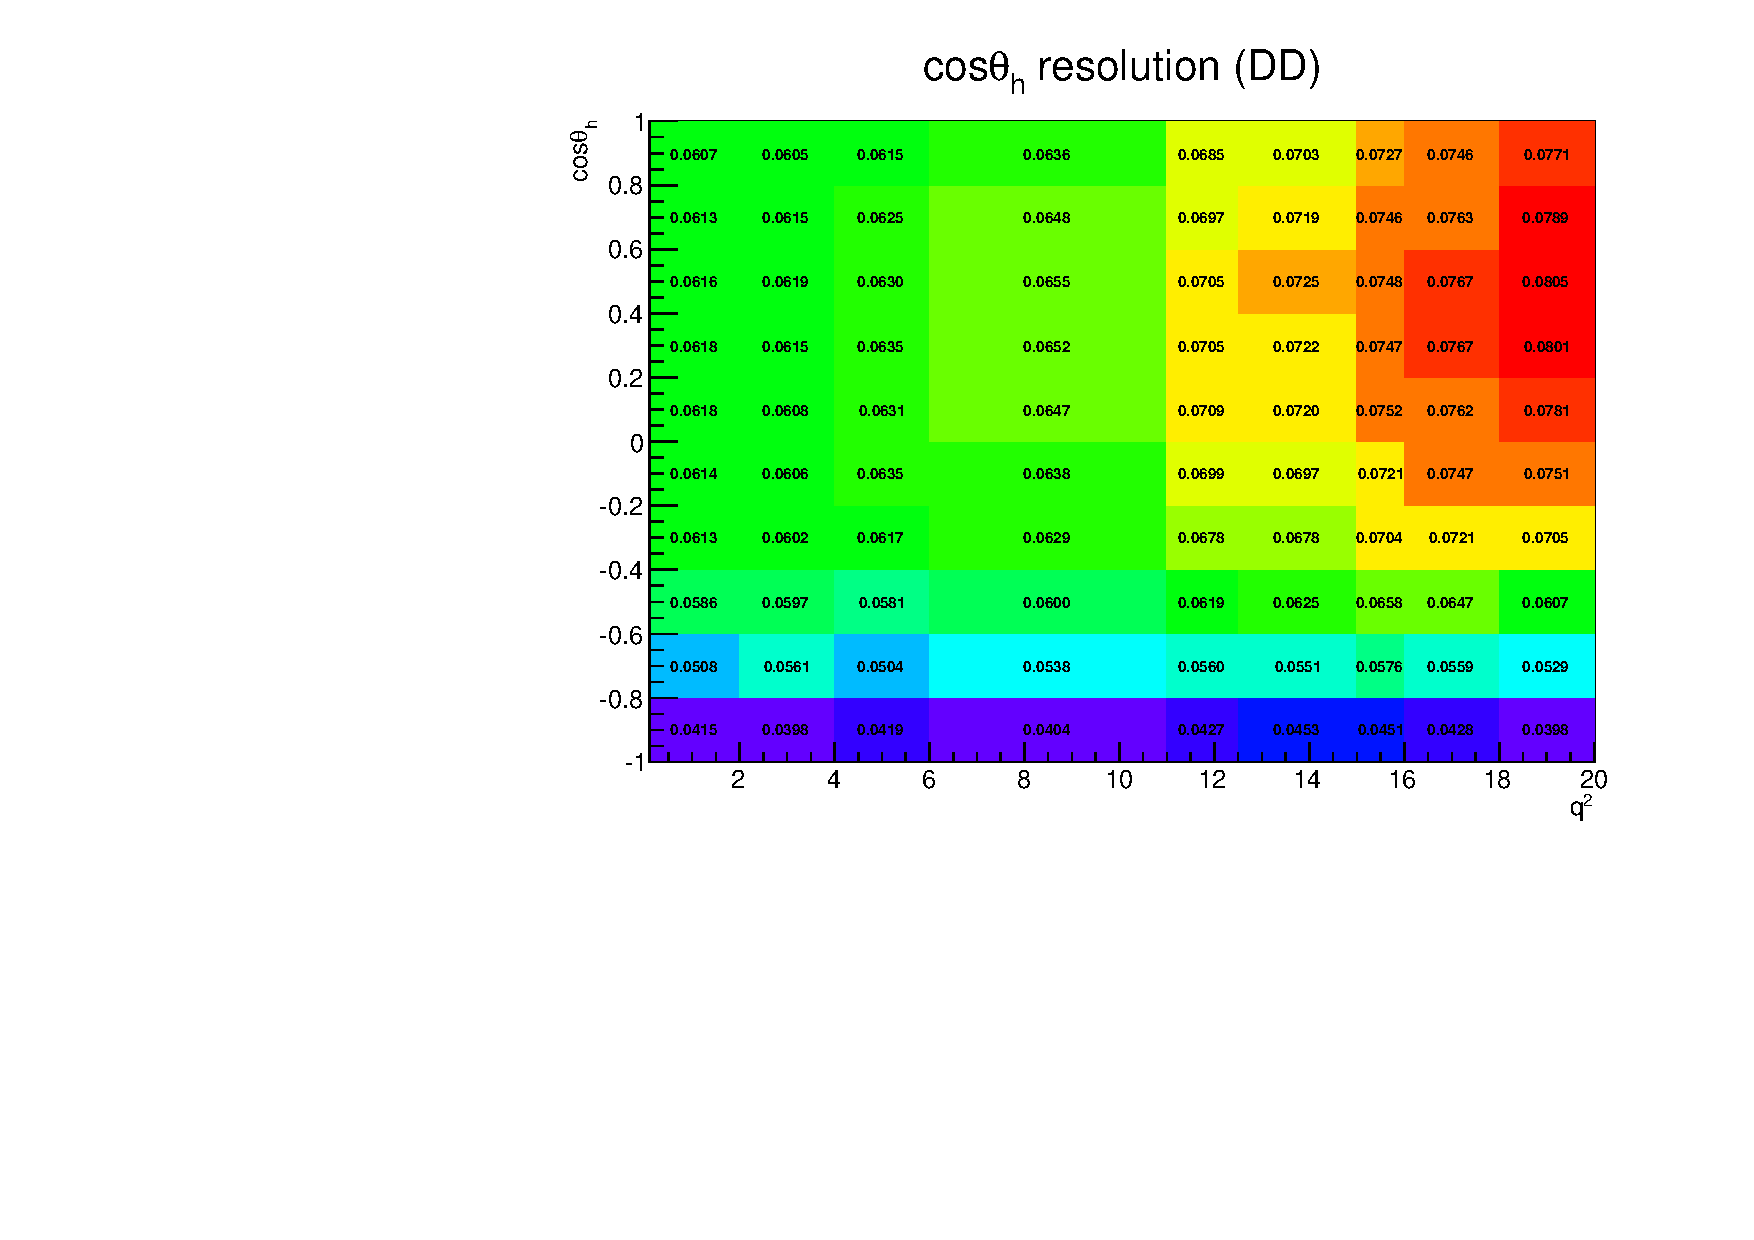
\includegraphics[width=0.48\textwidth]{Lmumu/figs/resolution/resolution2D_cosThetaB_DD.pdf} \\
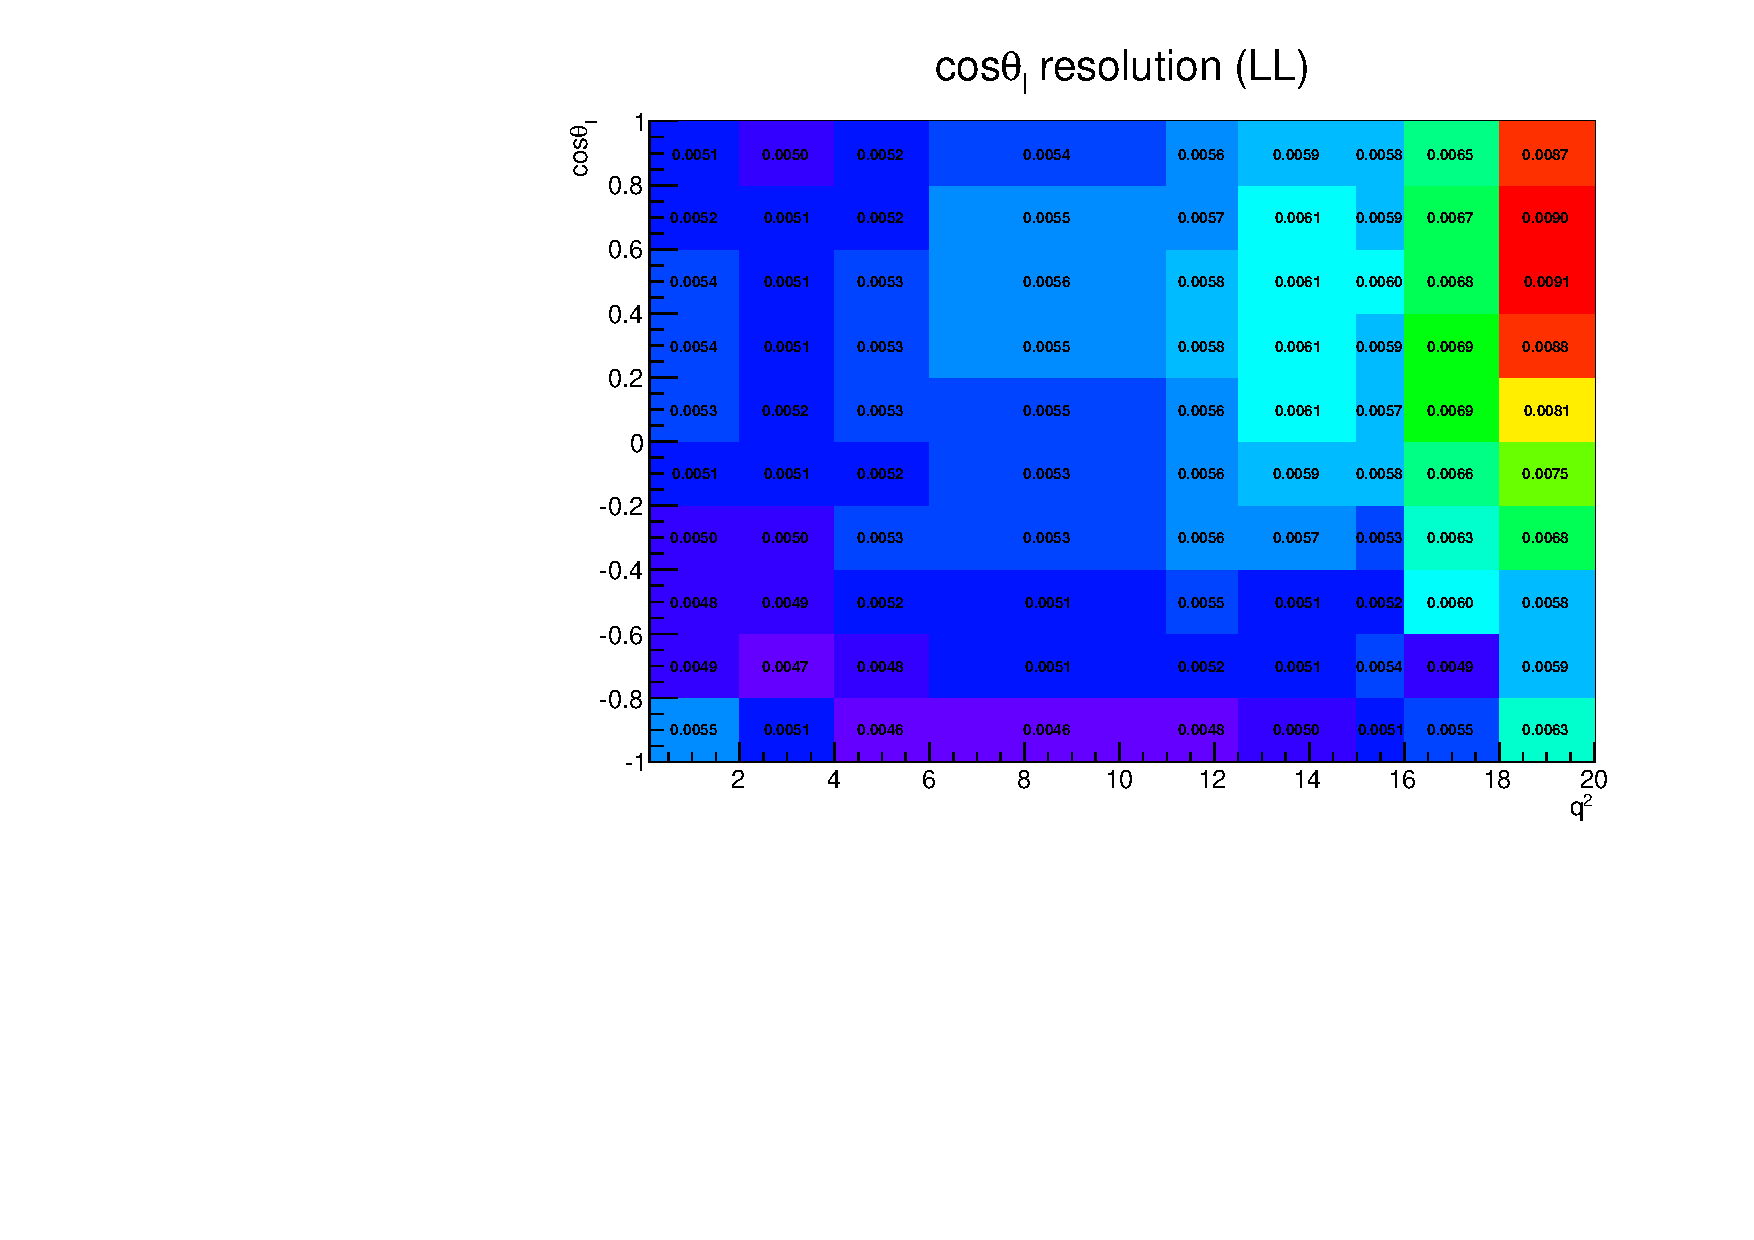
\includegraphics[width=0.48\textwidth]{Lmumu/figs/resolution/resolution2D_cosThetaL_LL.pdf}
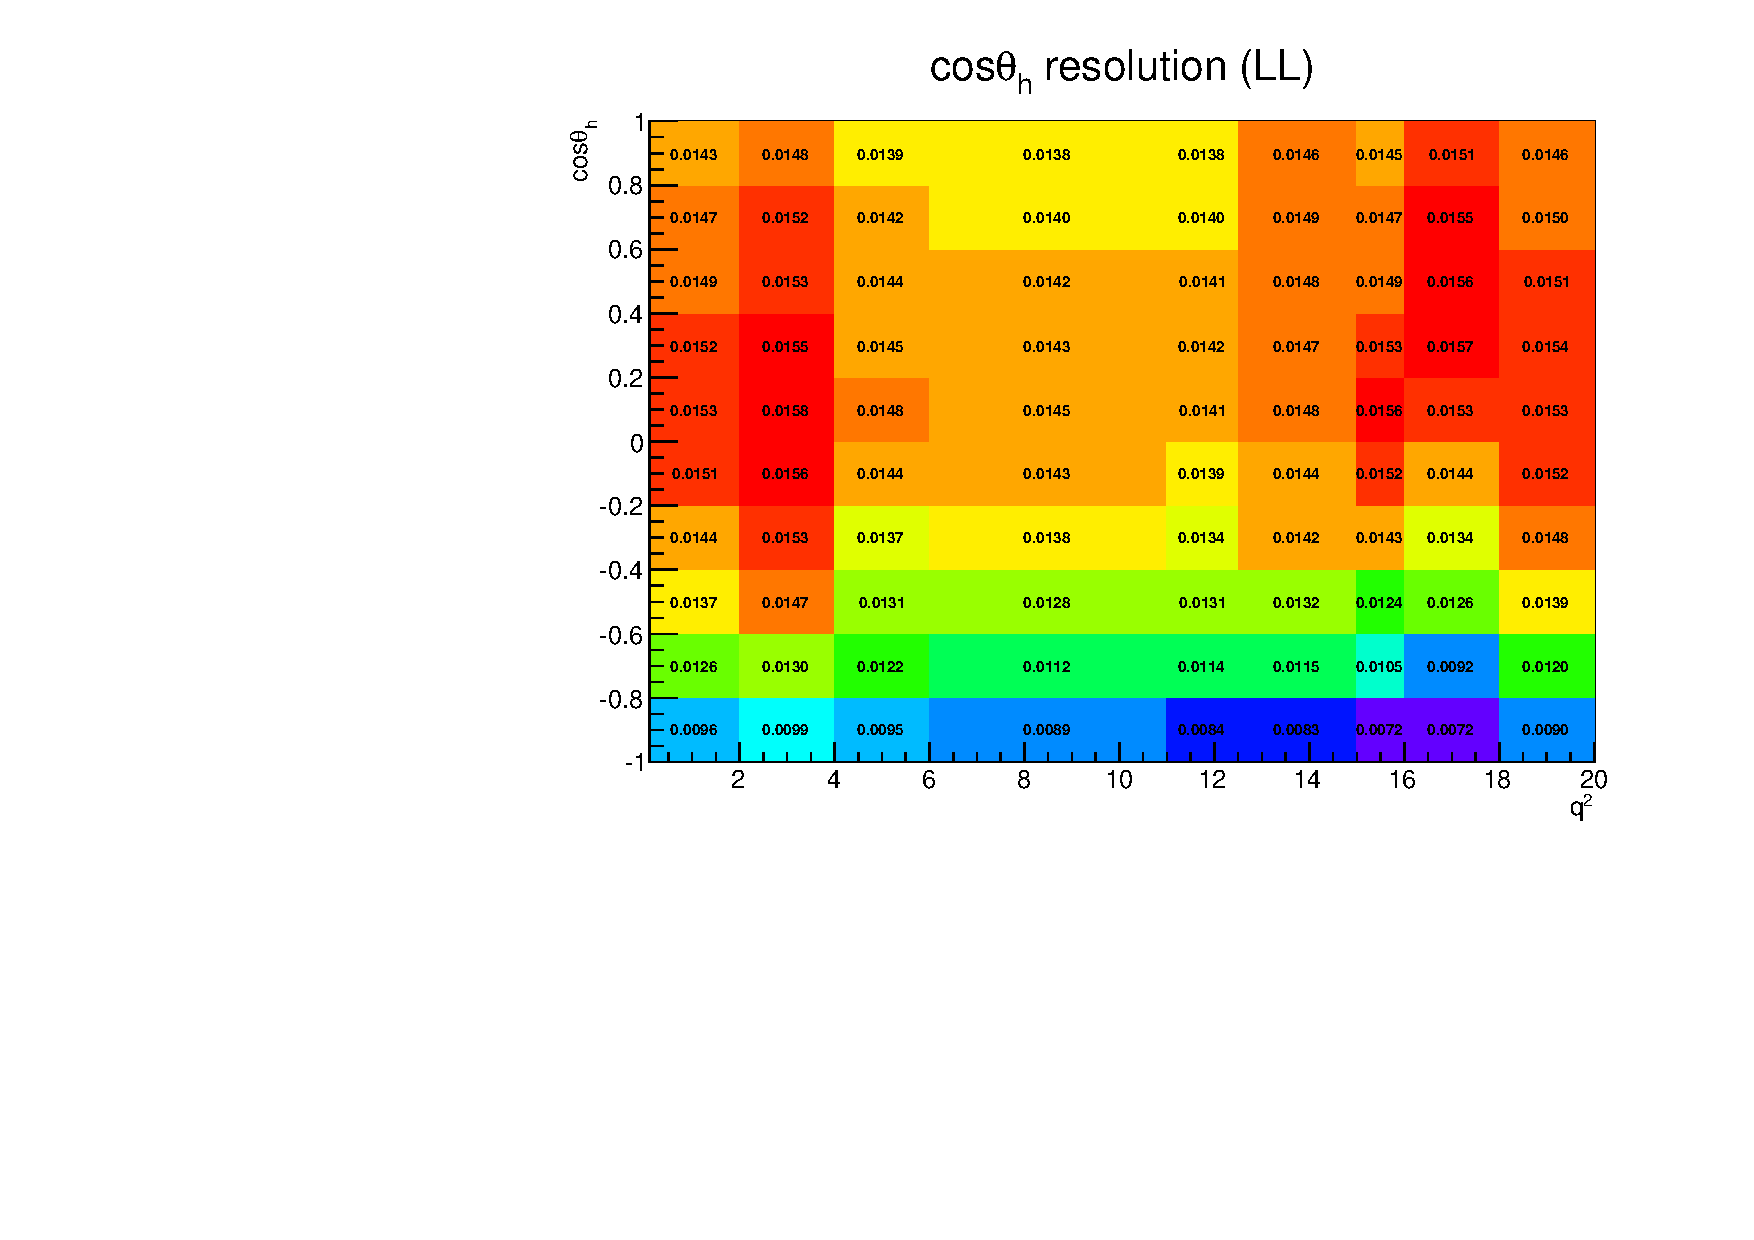
\includegraphics[width=0.48\textwidth]{Lmumu/figs/resolution/resolution2D_cosThetaB_LL.pdf}
\caption{Angular resolution for $\cos \theta_\ell$ (left plots) and  $\cos \theta_h$ (right plots)
as a function of the angular variables and \qsq for downstream (upper plots) and
long (lower plots) candidates. White bands correspond to the \jpsi and \psitwos resonances
which are excluded from the study.}
\label{fig:avgResol}
\end{figure}


